%\documentclass[11pt]{article}
%\usepackage{geometry}                % See geometry.pdf to learn the layout options. There are lots.
%\geometry{letterpaper}                   % ... or a4paper or a5paper or ...
%%\geometry{landscape}                % Activate for for rotated page geometry
%%\usepackage[parfill]{parskip}    % Activate to begin paragraphs with an empty line rather than an indent
%\usepackage{graphicx}
%\usepackage{amssymb}
%\usepackage{epstopdf}
%\usepackage{amsfonts}
%\usepackage{amsthm}
%\usepackage{amsmath}
%\usepackage{tikz}
%\usepackage{algorithm2e}
%\usepackage{url}
%\usepackage{comment}
%
%\newcommand{\mdp}{\mathcal{M}}
%\newcommand{\Mdp}{\mathcal{M}}
%\newcommand{\Agent}{\mathcal{G}}
%\newcommand{\env}{\mdp}
%\newcommand{\Env}{\mdp}
%\newcommand{\Actions}{\mathcal{A}}
%\newcommand{\action}{a}
%\newcommand{\actionp}{a^{\prime}}
%\newcommand{\actionpp}{a^{\prime\prime}}
%\newcommand{\States}{\mathcal{S}}
%\newcommand{\state}{s}
%\newcommand{\statep}{\state^{\prime}}
%\newcommand{\statepp}{\state^{\prime\prime}}
%\newcommand{\eststate}{x}
%
%\newcommand{\obs}{o}
%\newcommand{\Obs}{\mathcal{O}}
%\newcommand{\reward}{r}
%\newcommand{\terminalreward}{r^T}
%\newcommand{\rew}{\reward}
%\newcommand{\Rewards}{\mathcal{R}}
%\newcommand{\history}{h}
%\newcommand{\histories}{\mathcal{H}}
%\newcommand{\Histories}{\mathcal{H}}
%\newcommand{\Trans}{T}
%\newcommand{\Horizon}{t_f}
%\newcommand{\TUtility}{U_T}
%\newcommand{\Utility}{U_{\gamma}}
%\newcommand{\AUtility}{U_A}
%\newcommand{\TValue}{J}
%\newcommand{\TAValue}{K}
%\newcommand{\Value}{V}
%\newcommand{\hatValue}{{\widehat{V}}}
%\newcommand{\AValue}{Q}
%\newcommand{\hatAValue}{{\widehat{Q}}}
%\newcommand{\AvgRValue}{\rho}
%\newcommand{\hatAvgRValue}{{\widehat{\rho}}}
%\newcommand{\RelValue}{W}
%\newcommand{\hatRelValue}{{\widehat{W}}}
%
%\newcommand{\stateestfunction}{f_{su}}
%\newcommand{\stateobsfunction}{f_{so}}
%\newcommand{\statetransfunction}{f_{ss}}
%\newcommand{\rewfunction}{f_r}
%\newcommand{\field}[1]{\mathbb{#1}}
%\newcommand{\Reals}{\field{R}}
%%\newcommand{\eqref}[1]{(\ref{#1})}
%\newcommand{\policy}{\pi}
%\newcommand{\hatpolicy}{{\widehat{\pi}}}
%\newcommand{\Policies}{\Pi}
%\newcommand{\nspolicy}{\mu}
%
%\newcommand{\union}{\ensuremath{\bigcup}}
%\newcommand{\comps}{\ensuremath{\mathbb{C}}}
%\newcommand{\reals}{\ensuremath{\mathbb{R}}}
%\newcommand{\Var}{\ensuremath{\mathrm{Var}}}
%\newcommand{\var}{\ensuremath{\mathrm{Var}}}
%\newcommand{\E}{\ensuremath{\mathbb{E}}}
%\renewcommand{\P}{\ensuremath{\mathbb{P}}}
%\newcommand{\R}{\ensuremath{\mathbb{R}}}
%\newcommand{\Z}{\ensuremath{\mathbb{Z}}}
%
%\newcommand{\mixtime}{\tau}
%\newcommand{\epshorizon}{\tau}
%
%\def\argmax{\operatornamewithlimits{arg\,max}}
%\def\argmin{\operatornamewithlimits{arg\,min}}
%
%\newcommand{\bydef}{\stackrel{\bigtriangleup}{=}}
%\newcommand\defeq{\stackrel{\mathrm{def}}{=}}
%\newcommand{\half}{\frac{1}{2}}
%
%\DeclareGraphicsRule{.tif}{png}{.png}{`convert #1 `dirname #1`/`basename #1 .tif`.png}
%
%\newtheorem{proposition}{Proposition}
%\newtheorem{corollary}{Corollary}
%\newtheorem{assumption}{Assumption}
%\newtheorem{lemma}{Lemma}
%\newtheorem{definition}{Definition}
%\newtheorem{theorem}{Theorem}
%\newtheorem{example}{Example}
%\newtheorem{exercise}{Exercise}
%\newtheorem{remark}{Remark}
%
%\title{Lecture 1 - Introduction and Overview}
%\date{}                                           % Activate to display a given date or no date
%
%\begin{document}
%\maketitle
\section{Sequential Decision Problems}
The focus of this course is the solution of \emph{sequential decision problems}.  In such problems, a sequence of decisions is required, where each one has partial effect on the outcome.
Sequential decision problems are common in a wide variety of application domains, that include:
\begin{itemize}
  \item Artificial intelligence: Robotic motion planning, mission planning, board games (chess, backgammon), computer games (game of strategy, football).
  \item Operations research:  Inventory control, supply chain management, project assignment, scheduling of servers and customers.
  \item Finance: Investment strategies, financial planning, gambling.
  \item Communication networks and computer systems: Packet routing, flow control, cache handling, job scheduling, power control.
  \item Control Engineering: High-level feedback control of dynamic systems such as land/sea/air vehicles, chemical processes, power systems, analog amplifiers, etc.
\end{itemize}

We will examine two basic challenges in the context  of these decision problems:
\begin{enumerate}
  \item \textbf{Planning}: Optimal selection of the required sequence of actions (called an optimal control policy) to minimize a specified cost function in a given system model, when the model is \emph{known in advance}.
  \item \textbf{Learning}: When a system model is not available for the planner, it may need to be learned during operation, by trying out different options and observing their consequences.
\end{enumerate}

Our main \emph{planning} tools will rely on the theory of \emph{Dynamic Programming} (DP), which offers a set of methods and algorithms for solving sequential decision problems.

\emph{Reinforcement Learning} (RL) is the area of machine learning that deals with learning by observing the consequences of different actions. The term, which is borrowed from the behaviorist school in psychology, hints to the use of positive reinforcement to encourage certain behaviors. It is now used in machine learning to refer generally to learning in sequential decision processes and dynamical systems.

\paragraph{The situated agent viewpoint:} A basic viewpoint that underlies the field of RL, especially within AI, is that of the situated agent. The agent here may be a cognitive entity or a computer algorithm. It interacts with an external environment (the controlled system) by observing the environment state, and taking actions. Once an action is taken a reward signal is obtained, the system moves to a new state, and the cycle is repeated.
Designing an effective generic learning agent in such a framework may be seen as an ultimate goal in AI, and is a major driver of RL research.

\begin{figure}
  % Requires \usepackage{graphicx}
  \begin{centering}
  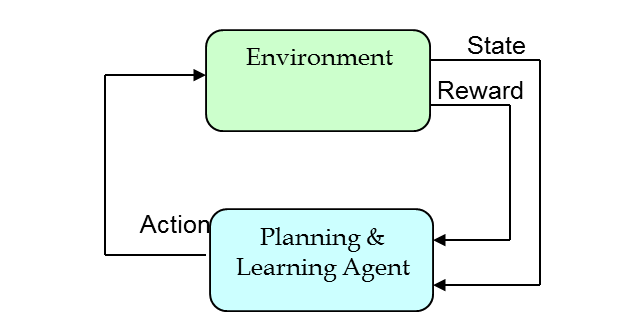
\includegraphics[width=0.5\textwidth]{lecture1_situated_agent}\\
  \caption{The situated agent}\label{fig:situated_agent}
  \end{centering}
\end{figure}

\begin{example}{\textbf{The Tetris player}}

Consider designing an AI player for the game of Tetris. The environment here would be the game simulator, and the environment state at a particular time corresponds to the game board at that time, and the shape of the new piece that just arrived. Upon observing a system state, the agent (the AI player) takes an action - it decides where on the board to position the new piece. Consequentially, if rows on the board were cleared, the agent receives a corresponding reward, and the the next system state is determined by the simulator.
\end{example}

\emph{Markov Decision Processes} (MDPs) are the standard model that allows to treat these planning and learning problems in a unified manner. An MDP describes a sequential decision problem, with the following properties:
\begin{itemize}
  \item A controlled dynamical system, with state-based dynamics. At each state some decision (or action) needs to be taken, and as a consequence the system moves to the next state.
  \item A reward function is associated with state-action pair, and the system performance is measured by the accumulated rewards.
  \item MDPs are especially suited to handle discrete problems (discrete state space, discrete action set, discrete time).
  \item MDPs allow to model in a natural way stochastic effects, and in particular stochastic system dynamics. We note that MDPs are currently the standard model for probabilistic planning in AI.
\end{itemize}

\subsection*{Challenges - what makes the planning problem hard?}
\begin{itemize}
  \item Lack of a global structure - most systems of interest do not have a simple global structure (such as that of a linear system). Therefore, planning needs to address each state (or group of states) in a distinct way.
  \item Large state-spaces: Many problems of interest have a huge number of states (recall the tetris example - how many board configurations are possible?), which makes exact solution impossible, even with the strongest algorithms.
        \emph{We note that models with a large number states are often the result of  combinatorial explosion in state vectors with a large number of components. This phenomenon is commonly known as the curse of dimensionality.}
  \item Large action-spaces: Some problems, especially in resource allocation, also exhibit large action-spaces, which present additional computational challenges.
  \item Stochastic effects - these are successfully handled within the MDP model, although they may add to the computational challenge.
  \item Uncertain or unknown environments -- which leads to the application of Reinforcement Learning techniques.
\end{itemize}

The computational challenge of complex problems (in particular, large state spaces) requires the use of approximation techniques for planning. This is an active research field, which is called Approximate Dynamic Programming (ADP) in our context. It is interesting to note that Reinforcement Learning techniques are often used as a means for planning in complex systems, even if the system dynamics is known.

The following diagram illustrates the relation and influence between the different disciplines involved.

  \begin{centering}
  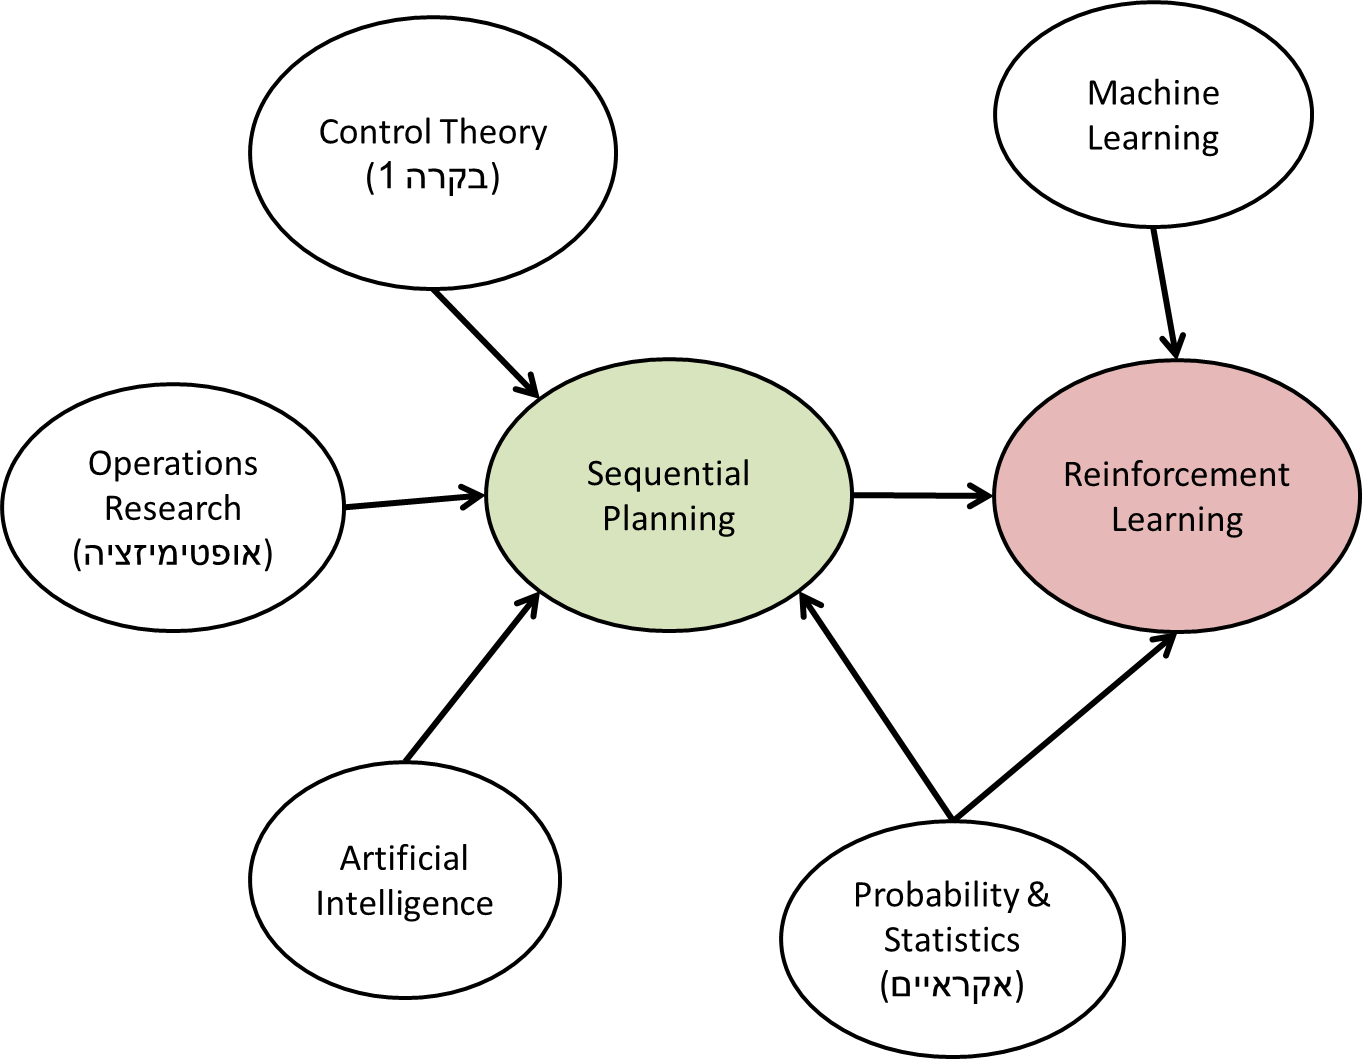
\includegraphics[width=0.7\textwidth]{lecture1_disciplines}\\
  \end{centering}

\section{Some Illustrative Planning Examples}
We next provide several examples that serve to illustrate the models involved. We start with planning examples.

\subsection{Shortest Path on a Graph}
Finding a shortest path between a source and destination nodes (or vertices) on a weighted graph is a generic problem with numerous applications, from routing in communication networks to trajectory planning, puzzle solving, and general AI planning. Essentially, Dynamic Programming based algorithms compute the distance from every node in the graph to the destination, spreading out from the destination until the source is reached. Specific algorithms for this problem include the Bellman-Ford algorithm, and Dijkstra's algorithm and its variants, such as A*.
This problem is widely discussed in courses on AI, and we will only briefly touch upon the main algorithms. We will also consider its stochastic generalization, the Stochastic Shortest Path problem.

\subsection{The Secretary Problem}
\paragraph{Problem setup:} We are interviewing $n$ candidates for a job. We know that the candidates are strictly ordered in quality from $1$ to $n$, but interview them in random order. Once we interview a candidate, his or her quality can be evaluated \emph{relative} to previously interviewed candidates. A candidate that is not hired during the interview cannot be recalled.
\paragraph{The planning problem:} Our goal is to find a rule for choosing a candidate, that will  maximize the chances of hiring the best one.

This problem and its generalizations have been widely studied in the operation research and computer science literature. It is an instance of a wider class of \emph{optimal stopping problems}.

\begin{exercise}
Let $B_t\sim \textrm{Bernoulli} $ i.i.d. for all $t=1,2,3,\dots$.
Consider the empirical average:
\begin{equation*}
    X_\tau = \frac{1}{\tau}\sum_{t=1}^{\tau} B_t.
\end{equation*}
where $\tau$ is a stopping time. The objective is to find a stopping rule for $\tau$ that maximizes $\mathbb E [X_\tau]$.
\begin{enumerate}
  \item Find a stopping rule that achieves $\mathbb E [X_\tau] \geq 0.75$
  \item (Hard!) What is the maximal $\mathbb E [X_\tau]$ that can be achieved?
\end{enumerate}
\end{exercise}

\subsection{Inventory Management}
\paragraph{System description:} Suppose we manage a single-item inventory system with daily orders. On the morning of each day $k$, we observe the current inventory ${x_k}$, and can order any quantity ${a_k} \ge 0$ of that item that arrives immediately. The daily demand for the item is denoted ${D_k}$. Thus, the number of items sold on each day $k$ is $\min \{ {D_k},{x_k} + {a_k}\} $, and the inventory at the end of the day is ${x_{k + 1}} = {[{x_k} + {a_k} - {D_k}]^ + }$. In this model we can determine the order $a_k$, whereas the demand $D_k$ is uncertain and is modeled as a random variable with known probability distribution. We assume that $D_k$ is a sequence of \emph{independent} random variables.

\paragraph{Cost structure:} Suppose that the cost for an order of $a_k$ is $J(a_k)$, a price $P$ is charged for each sold item, and a penalty $C({x_k} + {a_k} - {D_k})$ is incurred for over or under demand miss (where $C(y) \ge 0$ and  $C(0) = 0$).   Therefore, the net return (or reward) for day $k$ is \[{R_k} = P\,\min \{ {D_k},{x_k} + {a_k}\}  - J({a_k}) - C({x_k} + {a_k} - {D_k}).\]

The \emph{cumulative return} is the sum of daily returns over a given period, say $1$ to $K$.

\paragraph{The planning problem:} For each $k = 1, \ldots ,K$, we observe the current inventory $x_k$, and need to determine the amount $a_k$ to order next. The goal is to maximize the \emph{expected value} of the cumulative return over the given period:
\[E(\sum\nolimits_{k = 1}^K {{R_k}} )\; \to \;\min \]

\begin{remark}: A common policy in inventory management is the $(s,S)$ replenishment policy: whenever the inventory $x$ drops below $s$, order $S-x$ items. This policy can be shown to be optimal under appropriate assumptions on the cost.
\end{remark}
\begin{exercise} For the single-stage problem $(K=1)$  with $R=0$, $J\equiv0$, $C(y)=y^2$, show that a $(s,S)$ policy is optimal (with $s=S$).
\end{exercise}

\subsection{Admission control to a queueing system}
\paragraph{System description:} Consider a single-server queue, to which jobs (or customers) arrive sequentially. Each job has a service demand (in time unit of service) that is represented by a random variable with known distribution. The arrival process is, say, Poisson with rate $\lambda$.  The system manager can deny admission to an arriving job.

\paragraph{Cost structure:} Suppose that the system incurs a penalty of $C$ per unit time for each job waiting in the queue, and a reward $R$ for each customer served. We wish to minimize the expected cumulative cost over a period of time.

\paragraph{The planning problem:} Suppose a job arrives when the queue size is $x\geq0$. Should it be admitted or denied entry?
This problem represents a basic example of \emph{queueing control problems}. A wide range of computer, communication, and service systems can be represented by networks of queues (waiting lines) and servers. Efficient operation of these systems gives rise to a wide range of dynamic optimization problems. These include, among others, job admission control, job routing, server and job scheduling, and control of service rates.

\subsection{Stochastic scheduling}
\paragraph{System description: } Suppose we have a single server that caters to $n$ classes of jobs, one job at a time. Here the server may be human, a router in a communication network, a CPU in a computer system, etc. Jobs of class $i$ arrive as a Poisson process with rate $\lambda_i$, and each requires a service duration $D_i$ (which could be random -- for example, an exponentially-distributed random variable with expected value $\mu _i^{ - 1}$).

\paragraph{Cost structure:} Jobs of class $i$ incur a waiting cost  $C_i$ per unit time of waiting for service, and a reward $R_i$ for completing service.

\paragraph{The planning problem:} Suppose that the server becomes available at an instance $t$, and sees the state vector $X(t) = ({x_1}(t), \ldots ,{x_n}(t))$, where $x_i$ is the number of class $i$ jobs waiting for service. Which job class should the server attend next?

\section{Some Illustrative Learning Examples}
The following examples address the learning problem.

\subsection{The Multi-Armed Bandit (MAB) problem}
This is an important problem in statistics and machine learning. The exotic name derives from casino-like slot machines, which are also known as "single-armed bandits".
Suppose we are faced with $N$ different arms (slot machines), which may have different win probabilities (for simplicity assume 0-1 results, with obvious generalizations). These probabilities are not known to us.
There are two different goals in this problem:
\begin{enumerate}
  \item To identify the best arm (pure exploration).
  \item To maximize our gains over a large time horizon (exploration vs. exploitation).
\end{enumerate}

This model, under the second objective, presents in its purest form the \textbf{exploration vs. exploitation dilemma}, which is fundamental in Reinforcement Learning: While each arm may be optimal and should be sufficiently tried out, we should also focus at some point on the arm that seems to be the best. This tradeoff must be addressed by an appropriate  \emph{exploration strategy}.

We note that this problem can be considered as a special case of the MDP model, with a single state (i.e., static environment). Its original motivation was related to experimental drug (medicine) administration. Its current popularity in Machine Learning owes to recent on-line application such as ad posting: choosing the right class of ads to post in a given space or context to maximize revenue (or "click" count).

\subsection{Learning to Play Chess / Backgammon}
Current AI programs for chess playing essentially rely on extensive search in the game tree, starting from the current board position. That search is aided by an evaluation function (the \emph{heuristic}, or \emph{value function}), which provides a numerical value to each board position that estimates its strength (say, the likelihood of a win).

Suppose for simplicity that the opponent's playing strategy is known, so that the problem reduces to a single-player planning problem. The problem, of course, is huge number of states (board positions), which rules out an exact and complete solution. Therefore, partial solutions guided by heuristic and empirical rules must be used.

Machine learning offers a set of tools to improve the performance of a given AI player, by data-based tuning key parameter of the algorithm. Such improvements are often imperative for achieving state-of-the-art performance. Specific topics in which RL techniques have been successfully applied include:

\begin{itemize}
  \item Value function learning (by self-play and record analysis).
  \item Powerful heuristics for guiding the tree search.
\end{itemize}
These techniques have been applied in the games of Backgammon, Chess, and recently Go and Poker.

\subsection{Skill Learning in Robotics}
Suppose we wish to program a robot to juggle a ball on a racket, or to walk efficiently. We can start by programming the robot as best we can, but in most cases we will not be able to obtain fully efficient operation that way, and many "fine tunings" will be required.  One of the major approaches for improvement is to equip the robot with learning capabilities, so that it can improve its performance over time.
We can distinguish here between two learning goals:
\begin{enumerate}
\item[a.] Short term learning, or adaptivity - adapting to changing environment conditions (such as the weight of the ball, wind, etc.).
\item[b.] Skill learning - acquiring and improving the basic capability to perform certain motions or tasks in an efficient manner.
\end{enumerate}

A major Reinforcement Learning approach to these learning problems is a set of methods called \emph{direct policy search}. Here the required task or motion is parameterized by a vector of continuous parameters, which are tuned by simulation or during actual operation using gradient-based methods.  We will touch upon this important topic towards the end of the course.

\section{Mathematical Tools}
We briefly mention the main mathematical tools that will be used throughout the course.
\begin{enumerate}
  \item Concentration inequalities
  \item MDPs - dynamic programming
  \item Optimization - algorithms and theory
  \item Generalization and risk (PAC)
  \item Approximation theory
  \item Convergence of stochastic processes
\end{enumerate}

%\end{document}

